\documentclass[12pt, letterpaper]{article}
\usepackage[titletoc,title]{appendix}
\usepackage{color}
\usepackage{booktabs}
\usepackage[usenames,dvipsnames,svgnames,table]{xcolor}
\definecolor{dark-red}{rgb}{0.75,0.10,0.10}
\definecolor{dark-blue}{rgb}{0.0,0.0,0.7}
\usepackage[margin=1in]{geometry}
\usepackage[linkcolor=dark-blue,
            colorlinks=true,
            urlcolor=blue,
            pdfstartview={XYZ null null 1.00},
            pdfpagemode=UseNone,
            citecolor={dark-blue},
            pdftitle={Propagation of Error}]{hyperref}
%\usepackage{biblatex}
\usepackage{multibib}
\newcites{sec}{Other Sources}
\usepackage{geometry} % see geometry.pdf on how to lay out the page. There's lots.
\geometry{letterpaper}               % This is 8.5x11 paper. Options are a4paper or a5paper or other...
\usepackage{graphicx}                % Handles inclusion of major graphics formats and allows use of
\usepackage{amsfonts,amssymb,amsbsy}
\usepackage{amsxtra}
\usepackage{natbib}
\usepackage{dcolumn}
\usepackage{longtable}
\usepackage{verbatim}
\setcitestyle{round,semicolon,aysep={},yysep={;}}
\usepackage{setspace}            % Permits line spacing control. Options are \doublespacing, \onehalfspace
\usepackage{sectsty}             % Permits control of section header styles
\usepackage{lscape}
\usepackage{fancyhdr}            % Permits header customization. See header section below.
\usepackage{url}                     % Correctly formats URLs with the \url{} tag
\usepackage{fullpage}       %1-inch margins
\usepackage{multirow}
\usepackage{rotating}
\setlength{\parindent}{3em}

\usepackage{float}

\usepackage[T1]{fontenc}
\usepackage{bm}
\usepackage{libertine}
\usepackage{dcolumn}
\usepackage{chngcntr}

% Caption
\usepackage[hang, font=small,skip=0pt, labelfont={bf}]{caption}
\captionsetup[subtable]{font=small,skip=0pt}
\usepackage{subcaption}

% tt font issues
% \renewcommand*{\ttdefault}{qcr}
\renewcommand{\ttdefault}{pcr}

\usepackage{lscape}
\renewcommand{\textfraction}{0}
\renewcommand{\topfraction}{0.95}
\renewcommand{\bottomfraction}{0.95}
\renewcommand{\floatpagefraction}{0.40}
\setcounter{totalnumber}{5}
\makeatletter
\providecommand\phantomcaption{\caption@refstepcounter\@captype}
\makeatother
\begin{comment}

setwd(paste0(githubdir, "niewenhuis/ms/"))
tools::texi2dvi("niewenhuis.tex", pdf = TRUE, clean = TRUE)
setwd(githubdir)

\end{comment}

\begin{document}
\title{\Large{Significant Error: Citations to Research With Publicized Statistical Errors}\footnote{We are grateful to Danielle Portnoy and Xiaoran Huang for assisting us with the research, and to Andrew Gelman, Kabir Khanna, and Daniel Stone for offering valuable comments. The data and scripts for replicating the analysis are posted at: \href{https://github.com/recite/sig_error}{https://github.com/recite/sig\_error}}\\\vspace{5mm}}

\author{Ken Cor\\
\and Gaurav Sood}
%\vspace{5mm}}
%\date{\normalsize{\today}}
\maketitle

\vspace{.2cm}
\doublespacing
\clearpage
%\renewcommand{\abstractname}{Summary}
%\begin{abstract}
\textbf{Summary.} Many claims in a scientific article rest on research done by others. But when the claims are based on flawed research, scientific articles spread misinformation. Using data from an article published in \textit{Nature Neuroscience}, highlighting a serious statistical error in articles published in prominent journals. Data suggest that problematic research was cited without noting concerns with the work \textit{more frequently} after the problem was publicized. Our results have implications for the design of scholarship discovery systems and scientific practice more generally.
\vspace{.2cm}\\
\singlespacing
%\end{abstract}
\textit{Keywords.} Citation Behavior, Retractions, Scientific Integrity, Scientific Misconduct, Scientometrics
\doublespacing
\clearpage

\section{Introduction}

Retractions are generally a result of serious scientific malpractice. Retractions are also easily identified. Because of these reasons, research on citations to problematic research focuses exclusively on citations to articles that have been officially retracted. However, by focusing on retractions alone, we miss the more common problem of citations to unretracted studies with major errors. For example, \citet{gelman2006} discuss a common statistical error where researchers treat differences between significant and non-significant results as significant without conducting the requisite statistical test. They describe a scenario where results from two independent studies report parameter estimates and standard errors of 25 $\pm$ 10 and 10 $\pm$ 10, respectively. The first result is significant at the 1\% level, while the second is non-significant. The finding is interpreted by many as evidence of a significant difference, but a basic calculation of the difference in the effects and its standard error tells a different story, $15 \pm \sqrt{10^{2} + 10^{2}}$, which is not significant at the conventional 95\% level.

\citet{nieuwenhuis2011} analyzed 157 behavioral, systems, and cognitive neuroscience articles that relied on such analysis and were published in journals like \textit{Nature}, \textit{Science}, \textit{Neuron}, and \textit{Journal of Neuroscience} between 2009 and 2010. They found that roughly half (79) of the articles made this error. Further, they found that the error had serious consequences for the results for approximately two-thirds of the studies that made the error. To date, none of the studies that \citet{nieuwenhuis2011} identified as problematic have been retracted. We assess whether the citation rate changes after the publication of \citet{nieuwenhuis2011}.

Formally, we hypothesize that: Articles identified by \citet{nieuwenhuis2011} as suffering from a general statistical error will receive fewer citations per year after the publication of  \citet{nieuwenhuis2011} vis-a-vis similar articles without the error.

\section{Research Design}
To estimate the impact of the publication of error on citation rates, we implement an event study design by tracking the citation rate a few years before and after the error is made public. Given long publication cycles and assuming the article would have been accepted for publication before the discovery of the error, we test the impact on citations one, two, and three years after the publication of the retraction notice. We also use a Difference-in-Differences estimator, exploiting the fact that roughly half of the articles published in the same journals did not make the same error. 

\section{Results}

Prima facie evidence suggests little impact of the publication of \citet{nieuwenhuis2011} on citations to articles mistaking the difference between significant effect and insignificant effect as evidence for a significant difference. In the two years before the publication of \citet{nieuwenhuis2011}, and the year \citet{nieuwenhuis2011} was published (2011), the 79 articles making the mistake were cited 2,267 times. Between 2012 and 2015, the articles were cited an additional 6,604 times.

Figure \ref{fig:niewenhuis} offers a closer look. It plots the total number of citations received per year by each of the papers making the mistake, the average number of citations received per year by articles making the mistake, and smoothed \texttt{loess} growth curves. The plot also shows there is a skew in citation rates (skewness based on the method of moments = 2). To account for the skew, we switched means with medians. Doing so yields a pretty similar pattern except for the expected intercept shift (see Figure \ref{fig:median_niewenhuis}). Not all articles making the error, however, have results similarly affected by the error. Fortunately, \citet{nieuwenhuis2011} flag articles where the error has potentially serious consequences for the results. Thus, next, we track what happens to citations to such articles. We track how the median number of citations vary across years and whether they are affected by the publication of the \citet{nieuwenhuis2011}. As Figure \ref{fig:serious_niewenhuis} shows, the median number of citations steadily and modestly increase over time with the publication of \citet{nieuwenhuis2011}.

\begin{figure}[H]
\centering
 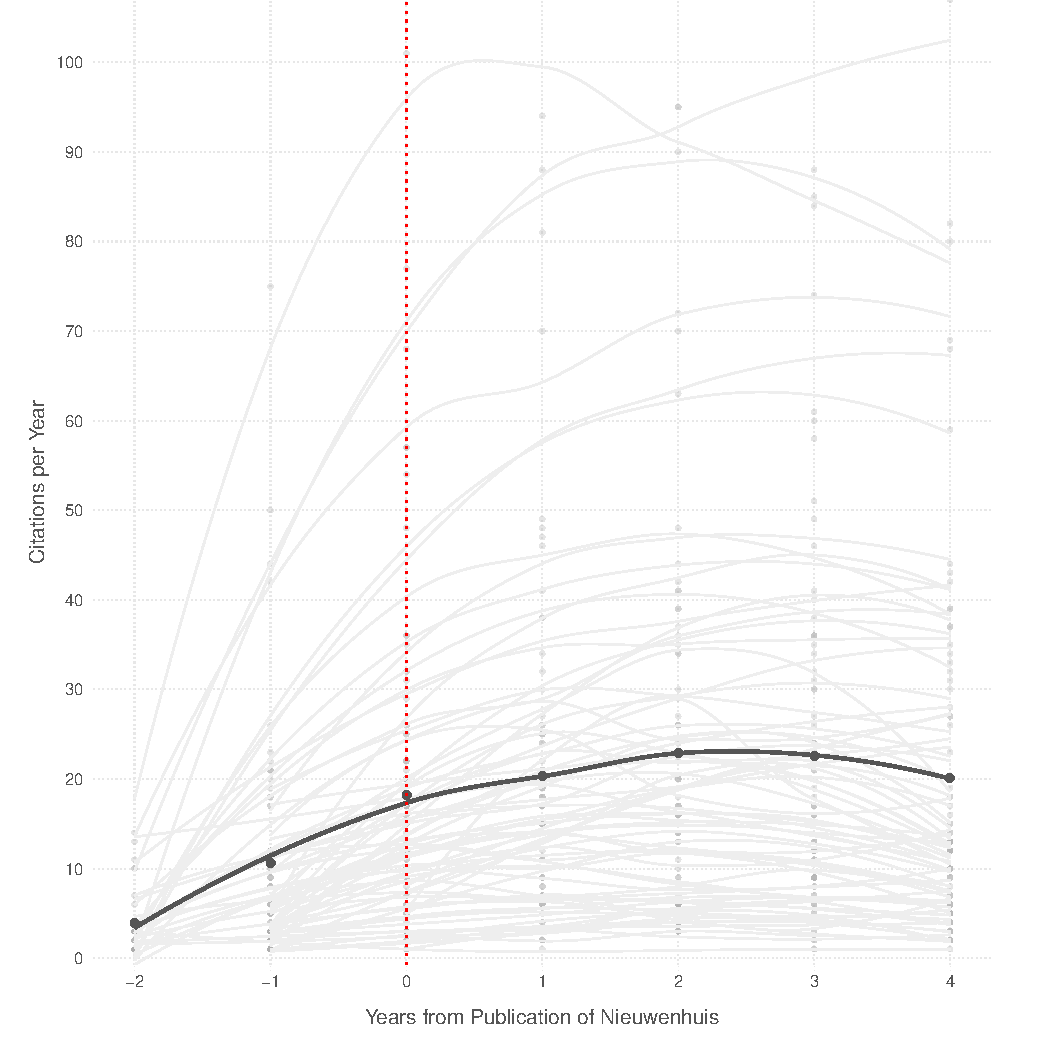
\includegraphics[scale=.7]{../figs/nw_growth_curve.pdf}
 \caption{Number of Citations to Articles Containing the Error Per Year}
 \label{fig:niewenhuis}
\end{figure}

To estimate the percentage of citations that do not acknowledge problems after the publication of Nieuwenhuis et al., we coded whether the citation acknowledged the problem or not in 100 randomly chosen articles citing articles with the mistake (see SI \ref{approving_or_not} for further details about how the citations were coded.) Of the 100, only one article noted concerns with the cited article, citing \citep{nieuwenhuis2011} for support.

To more formally explore the change in citation rate as a consequence of the publication of \citet{nieuwenhuis2011}, we regress citations per year on a dummy for the year \citet{nieuwenhuis2011} was published, a linear time trend, and fixed-effect for the article. We also cluster by articles to account for multiple observations per article. In effect, we are estimating an average of within article changes after regressing out a linear time trend as above. Results show, if anything, a modest uptick in citations after \citet{nieuwenhuis2011} is published---a year after the publication of \citet{nieuwenhuis2011}, articles containing the error get about four more citations per year compared to what they were getting before it (see Table \ref{tab:si_tab1}).

Our main analysis for the \citeauthor{nieuwenhuis2011} data is a Difference-in-Differences (DID) analysis. DID gives us a better way to control for over time trends. We estimated whether the difference in citation rates of articles making the error and those not making the error changed after the publication of \citet{nieuwenhuis2011}. In particular, letting $i$ index articles and $j$ index years, we regressed citations per year ($y_ij$) on whether or not the article makes the error ($s_i$), years to the publication of \citeauthor{nieuwenhuis2011} ($n_i$) and an interaction between the two. Again, we clustered the standard errors by article. In all, we estimated the following model:

\begin{align}
\label{eqn:eqn2}
y = \alpha + \beta_1 n_i + \beta_2 s_i + \beta_3 (n*s) + \epsilon
\end{align}

Table \ref{tab:tab1} tabulates the results. Models (1), (3), and (5) define error as all articles making the error. Models (2), (4), and (6) refer to error as articles making ``potentially serious errors.'' As the table shows, 1 or 2 years after \citet{nieuwenhuis2011}, articles making the error were being cited more frequently vis-\`a-vis articles not making the error (Diff. $\sim$ 3). Three years out, we cannot still reject the 0, suggesting that there is no evidence of a decline. For articles making ``potentially serious errors'', the story is much the same, except that the one and two-year out estimates are closer to 3.5 additional citations per year than 3. Three years later, we still cannot say that the articles making ``potentially serious errors'' were being cited any less frequently.  In all, there is strong evidence that citations that do not acknowledge problems remain common after the error is publicized. The publicity of \citeauthor{nieuwenhuis2011} has had little impact, with articles containing errors still being highly cited. These articles may be especially susceptible to continued citations because the nature of the error results in an inference of a difference in differences that is something other researchers are looking for evidence of in order to support an important point.


% Table created by stargazer v.5.2.2 by Marek Hlavac, Harvard University. E-mail: hlavac at fas.harvard.edu
% Date and time: Fri, Feb 05, 2021 - 12:20:46 PM
% Requires LaTeX packages: dcolumn rotating 
\begin{sidewaystable}[!htbp] \centering 
  \caption{Difference-in-Difference Analysis of the Impact of Publication of Nieuwenhuis on the Number of Times per Year Articles Containing the Error Are Cited Vis-a-Vis Articles that Didn't Contain the Error} 
  \label{tab:tab1} 
\small 
\begin{tabular}{@{\extracolsep{5pt}}lD{.}{.}{-1} D{.}{.}{-1} D{.}{.}{-1} D{.}{.}{-1} D{.}{.}{-1} D{.}{.}{-1} } 
\\[-1.8ex]\hline 
\hline \\[-1.8ex] 
 & \multicolumn{6}{c}{\textit{Dependent variable:}} \\ 
\cline{2-7} 
\\[-1.8ex] & \multicolumn{6}{c}{Citations per year} \\ 
 & \multicolumn{2}{c}{1 year out} & \multicolumn{2}{c}{2 years out} & \multicolumn{2}{c}{3 years out} \\ 
\\[-1.8ex] & \multicolumn{1}{c}{(1)} & \multicolumn{1}{c}{(2)} & \multicolumn{1}{c}{(3)} & \multicolumn{1}{c}{(4)} & \multicolumn{1}{c}{(5)} & \multicolumn{1}{c}{(6)}\\ 
\hline \\[-1.8ex] 
 Treatment Date & 7.2^{***} & 7.7^{***} & 5.1^{***} & 5.5^{***} & 3.7^{***} & 3.9^{***} \\ 
  & (0.9) & (0.7) & (0.9) & (0.7) & (1.0) & (0.8) \\ 
  Error or Not & 1.5 & 0.004 & 2.1 & 0.6 & 2.8 & 1.6 \\ 
  & (2.5) & (2.8) & (2.4) & (2.7) & (2.4) & (2.6) \\ 
  Makes Error*Treatment Date & 3.1^{**} & 3.7^{***} & 2.7^{**} & 3.5^{***} & 1.7 & 2.1 \\ 
  & (1.2) & (1.3) & (1.2) & (1.3) & (1.3) & (1.5) \\ 
  Constant & 9.5^{***} & 10.2^{***} & 11.7^{***} & 12.6^{***} & 13.1^{***} & 14.0^{***} \\ 
  & (1.8) & (1.5) & (1.7) & (1.5) & (1.7) & (1.4) \\ 
 \hline \\[-1.8ex] 
Observations & \multicolumn{1}{c}{957} & \multicolumn{1}{c}{957} & \multicolumn{1}{c}{957} & \multicolumn{1}{c}{957} & \multicolumn{1}{c}{957} & \multicolumn{1}{c}{957} \\ 
Akaike Inf. Crit. & \multicolumn{1}{c}{7,328.2} & \multicolumn{1}{c}{7,327.8} & \multicolumn{1}{c}{7,408.8} & \multicolumn{1}{c}{7,407.5} & \multicolumn{1}{c}{7,474.9} & \multicolumn{1}{c}{7,475.2} \\ 
Bayesian Inf. Crit. & \multicolumn{1}{c}{7,357.4} & \multicolumn{1}{c}{7,357.0} & \multicolumn{1}{c}{7,437.9} & \multicolumn{1}{c}{7,436.7} & \multicolumn{1}{c}{7,504.0} & \multicolumn{1}{c}{7,504.4} \\ 
\hline 
\hline \\[-1.8ex] 
\textit{Note:}  & \multicolumn{6}{l}{$^{*}$p$<$0.1; $^{**}$p$<$0.05; $^{***}$p$<$0.01} \\ 
 & \multicolumn{6}{l}{Models (1), (3), and (5) define error as any article making the error.} \\ 
 & \multicolumn{6}{l}{And Models (2), (4), and (6) refer to error as articles making ``potentially serious errors.''} \\ 
\end{tabular} 
\end{sidewaystable} 



\clearpage
\bibliographystyle{rss}
\bibliography{error}

\clearpage
\appendix
\renewcommand{\thesection}{SI \arabic{section}}
\renewcommand\thetable{\thesection.\arabic{table}}
\renewcommand\thefigure{\thesection.\arabic{figure}}
\counterwithin{figure}{section}
\setcounter{figure}{0}
\setcounter{section}{0}
\setcounter{table}{0}

\begin{center}
\Large{Supporting Information}
\end{center}

\section{Rate of Citations Before and After Publication of Nieuwenhuis et al.}

\begin{figure}[H]
\centering
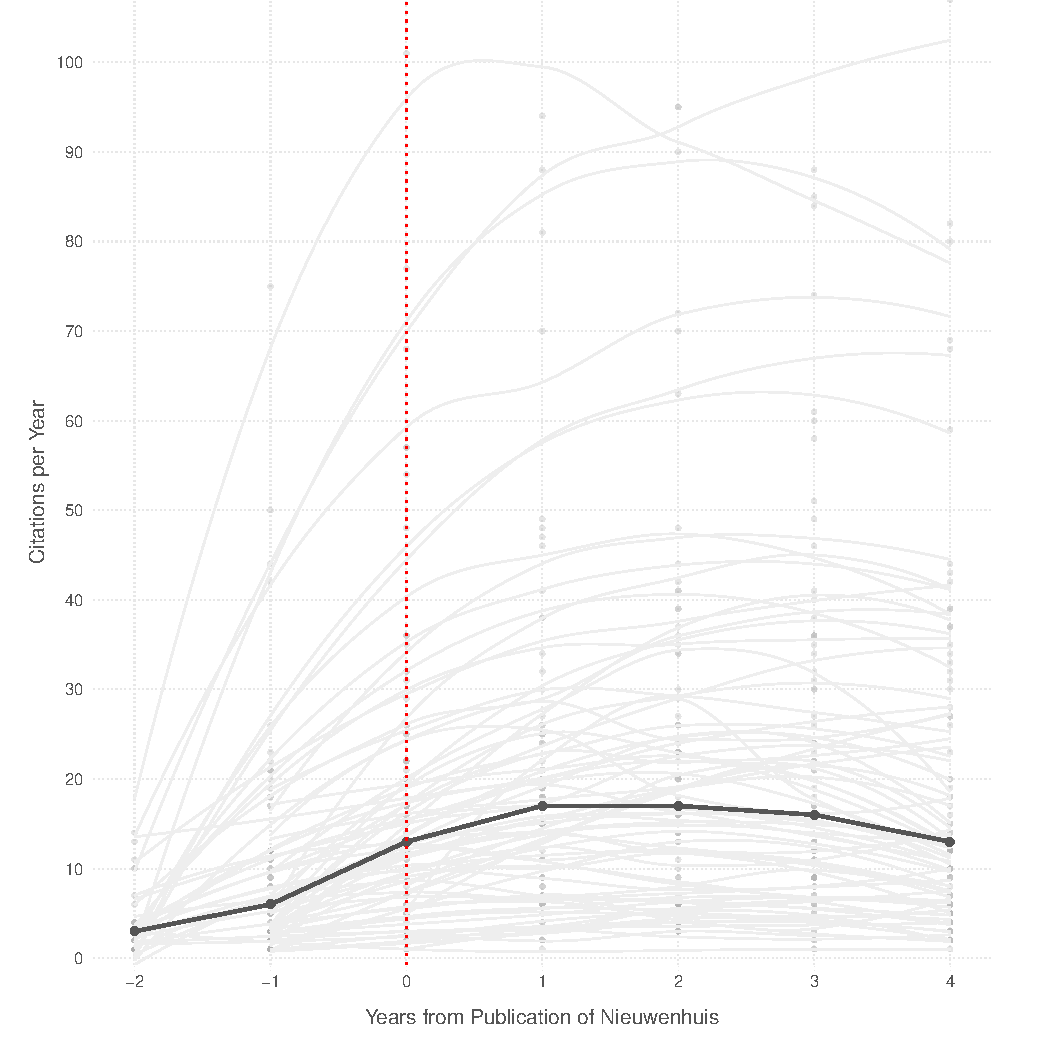
\includegraphics[scale=.7]{../figs/nw_median_growth_curve.pdf}
\caption{Total number of citations received per year by each of the papers making the mistake, and the median number of citations received per year by the articles.}
\label{fig:median_niewenhuis}
\end{figure}

\clearpage
\begin{figure}[H]
\centering
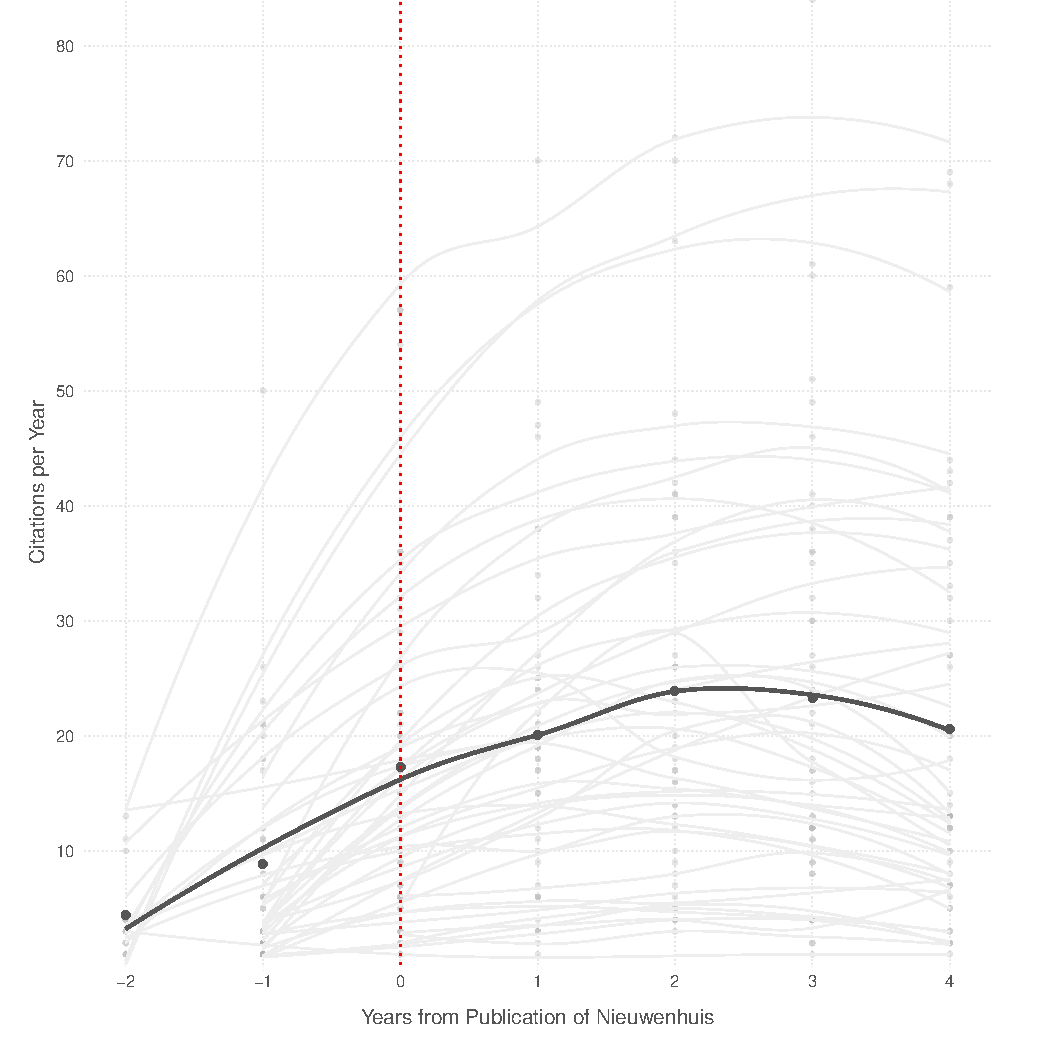
\includegraphics[scale=.7]{../figs/serious_nw_growth_curve.pdf}
\caption{Total number of citations received per year by articles making the mistake with `potentially serious' consequences for the results, and the average number of citations received per year by the articles.}
\label{fig:serious_niewenhuis}
\end{figure}

\clearpage

% Table created by stargazer v.5.2.2 by Marek Hlavac, Harvard University. E-mail: hlavac at fas.harvard.edu
% Date and time: Thu, Feb 11, 2021 - 11:42:46 PM
% Requires LaTeX packages: dcolumn 
\begin{table}[!htbp] \centering 
  \caption{Change in the Number of Citations to Articles Containing the Error Per Year Before and After Publication of Nieuwenhuis} 
  \label{tab:si_tab1} 
\begin{tabular}{@{\extracolsep{5pt}}lD{.}{.}{-1} D{.}{.}{-1} } 
\\[-1.8ex]\hline 
\hline \\[-1.8ex] 
 & \multicolumn{2}{c}{\textit{Dependent variable:}} \\ 
\cline{2-3} 
\\[-1.8ex] & \multicolumn{2}{c}{Citations Per Year} \\ 
 & \multicolumn{1}{c}{All Articles with Mistakes} & \multicolumn{1}{c}{Articles with Potentially Serious Errors} \\ 
\\[-1.8ex] & \multicolumn{1}{c}{(1)} & \multicolumn{1}{c}{(2)}\\ 
\hline \\[-1.8ex] 
 Transition Date & 3.8^{**} & 5.0^{**} \\ 
  & (1.7) & (2.0) \\ 
  Time & 2.0^{***} & 2.1^{***} \\ 
  & (0.4) & (0.5) \\ 
  Constant & 20.8 & 19.8 \\ 
  & (15.6) & (28.6) \\ 
 \hline \\[-1.8ex] 
Observations & \multicolumn{1}{c}{487} & \multicolumn{1}{c}{276} \\ 
Akaike Inf. Crit. & \multicolumn{1}{c}{3,322.0} & \multicolumn{1}{c}{1,827.1} \\ 
Bayesian Inf. Crit. & \multicolumn{1}{c}{3,665.4} & \multicolumn{1}{c}{2,004.5} \\ 
\hline 
\hline \\[-1.8ex] 
\textit{Note:}  & \multicolumn{2}{r}{$^{*}$p$<$0.1; $^{**}$p$<$0.05; $^{***}$p$<$0.01} \\ 
\end{tabular} 
\end{table} 


\clearpage
\section{Coding Citations as Acknolwedging Problems Or Not}
\label{approving_or_not}
To code the citations, we downloaded citing articles and their associated retracted article. A research assistant then edited the citing article pdf to highlight where the retracted article was discussed in the citing article. The judgment of whether the article noted any concerns was made based on a review of the original retracted article pdf and the highlighted text. 

If an article did not note any concerns with the cited article, it was coded as \textit{not acknoledging problems}. Simply disagreeing with the conclusions of an article without noting any concern still meant that the article was being cited in a way that suggests that its findings are trustworthy and were also coded as \textit{not acknowledging problems}. We code articles that note any concern with the citing article, even those unrelated to the cause of retraction, as \textit{acknowledging problems}. 

In the Nieuwenhuis data, we could not locate one of the 100 articles, leaving us with 99 articles. Of the 99 articles, 2 were false positives---the articles did not cite erroneous research, but instead cited a paper with authors and title similar to published erroneous research. Of the 97 remaining articles, only one article noted concerns while citing an article making a mistake, citing \citet{nieuwenhuis2011} for support. 

We evaluated the reliability of the coding by having an independent rater code 50 randomly selected citing articles. The two sets of independent codes were found to agree in all 50 instances.

\end{document}
